\subsection{Порождающие состязательные сети}
Порождающие состязательные сети (\texttt{Generative Adversarial Network}, \texttt{GAN}) "--- модель, предназначенная для генерации качественных изображений на основе существующего набора данных. Впервые была предложена в 2014 году в деятельности Иэна Гудфеллоу. Классическая реализация порождающих состязательных сетей состоит из двух искусственных нейронных сетей, цель которых "--- <<одолеть>> друг друга.

Одна из нейронных сетей в \texttt{GAN} называется генератором (generator) и предназначена для порождения объектов в пространстве данных, а вторая нейронная сеть является дискриминатором (discriminator). Задача дискриминатора заключается в классификации подаваемых на вход изображений, в том числе порожденных вышеописанным генератором. Таким образом, задача дискриминатора сводится к успешной классификации, а задача генератора "--- минимизировать оценивающую функцию дискриминатора \cite{gan_intro}.

Поскольку нейронные сети сами по себе не умеют генерировать новые примеры из ничего, необходимо, чтобы модели преобразовывали случайны входы из стандартного нормального распределения $\mathcal{N}(0, 1)$. Таким образом, нейронная сеть будет преобразовывать распределение $\mathcal{N}(0, 1)$ в распределение данных. Формально, генератор можно записать следующим образом:


\begin{equation}
    G = G(z; \theta_g): Z \rightarrow X,
\end{equation}
где $Z$ "--- пространство латентных факторов, где есть распределение $p_z(z)$. 

Дискриминатор выглядит следующим образом:
\begin{equation}
    D = D(x; \theta_d): X \rightarrow [0, 1]
\end{equation}
В данном случае, данные конвертируется в отрезок $[0, 1]$, который означает вероятность того, что поданный на вход пример не является выходом генератора. Таким образом, дискриминатор хочет максимизировать следующую величину:
\begin{equation}
    \mathbb{E}_{x \sim p_{data}(x)}[\log D(x)] + \mathbb{E}_{x \sim p_{gen}(x)}[1 - \log D(x)],
\end{equation}
где $p_{gen}(x)$ "--- элемент из порождаемого генератором распределения ,$p_{gen}(x) = G_{z \sim p_z}(x)$

В общем случае, генеративные состязательные сети решают задачу оптимизации, широко известную как <<задача minimax>>: \cite{nikolenko_dl}
\begin{equation}
    \min\limits_{G}\max\limits_{D}V(D, G),
\end{equation}
где
\begin{equation}
    V(D, G) = \mathbb{E}_{x \sim p_{gen}(x)}[\log D(x)] + \mathbb{E}_{z \sim p_{z}(z)}[1 - \log D(G(z))]
\end{equation}

Общий вид порождающих состязательных сетей (\texttt{pipeline}) можно рассмотреть на рисунке \ref{fig:gan_overview}\cite{gan_intro}.

\begin{figure}[H]
    \centering
    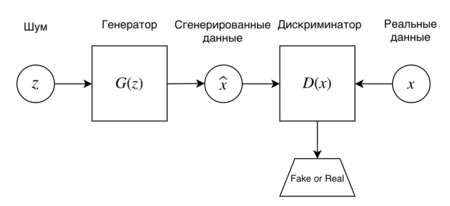
\includegraphics[width=0.7\linewidth]{images/gan_overview.png}
    \caption{Классическая реализация GAN}
    \label{fig:gan_overview}
\end{figure}

Общий процесс обучения модели относительно распределений данных можно увидеть на рисунке \ref{fig:gan_train} \cite{gan_intro}.
\begin{figure}[H]
    \centering
    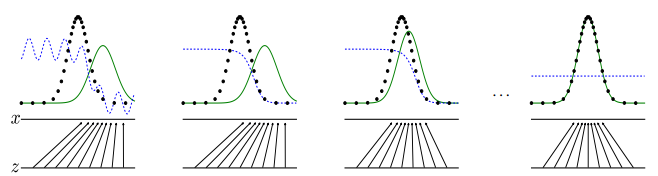
\includegraphics[width=0.9\linewidth]{images/gan_train.png}
    \caption{Процесс обучения: синяя пунктирная линия "--- дискриминантное распределение, чёрная пунктирная линия "--- порождающее распределение, зеленая сплошная линия "--- генеративное распределение, верхняя горизонтальная линия "--- часть области из $\mathbb{X}$, нижняя горизонтальная линия "--- область, из которой отбирается выборка $z$.}
    \label{fig:gan_train}
\end{figure}

Одним из недостатков архитектуры \texttt{GAN} является вероятное схлопывание в моду (mode collapse), когда генератор находит распределение, данные из которого дискриминатор не может корректно классифицировать. В этом случае существует вероятность, что генератор остановится в этом распределении и продолжит генерировать изображения, опираясь только на эту часть признакового пространства \cite{gan_intro}.

\subsubsection{Использование \texttt{GAN}}
При обучении, модели могут использовать парные и непарные изображения. В зависимости от этого параметра, задача ставится по"=разному. Для парных данных задача является обучением с учителем (supervised learning), поскольку у модели есть чёткое обозначение, на какую картинку по пикселям стоит ориентироваться. В то время как непарные данные являются обучением без учителя (unsupervised learning), то есть не существует чёткого обозначения, во что должно превратиться исходное изображение. С точки зрения качества изображения это может повлиять, однако вариант с задачей без учителя является более приблежённым к реальной жизни и именно на непарных данных обучаются модели для коммерческих целей \cite{unpaired}.

Рассмотрим применение порождающих состязательных сетей в коммерческой разработке. В рамках анализа было рассмотренно решение \texttt{PASTA"=GAN++}, использующее непарные изображения для обучения. Пусть $I_s$ "--- исходное изображение, модель на котором одета в бельё $G_s$. Задача виртуальной примерочной "--- сгенерировать изображение $I'_t$, являющееся копией изображения $I_t$ в одежде $G_s$. Для достижения данного результата, \texttt{PASTA"=GAN++} использует модуль распутывания с маршрутизацией патчей, результат работы которого можно увидеть на изображении \ref{fig:gan_prdm} \cite{pasta_gan}.
\begin{figure}[H]
    \centering
    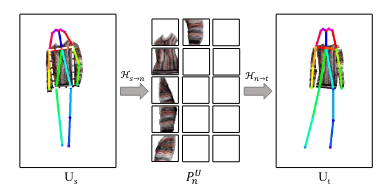
\includegraphics[width=0.6\linewidth]{images/gan_prdm_res.png}
    \caption{Модуль распутывания с маршрутизацией патчей}
    \label{fig:gan_prdm}
\end{figure}

Одежда $G_s$ преобразуется в патчи $P_n$, которые в свою очередь деформируются для перехода к деформированной одежде $G_t$. Таким образом, данный модуль делает некоторое предсказание позы человека, основываясь на нормализованных патчах. $G_t$ соответствует позе целевого человека.

Затем для генерации реалистичного результата примерки одежды, применяется модуль \texttt{StyleGAN2}, где происходит синтезация парсинга человека $S_t$. Данный парсинг отображает основные детали, такие как поза и одежда, чтобы на основе особенностей накладываемой одежды сделать нужные искажения.

Затем применяется модуль \texttt{Spatially-Adaptive Residual Module}, который встраивается в генератор \texttt{GAN} и который отвечает за наложение искажённой одежды на новую позу. Этот модуль использует метод inpainting и SPADE"=нормализацию для модуляции и визуализации полученных признаков \cite{pasta_gan} \cite{spade}.

При обучении \texttt{PASTA"=GAN++} в качестве функций потерь были использованы:
\begin{equation}
    L_{rec} = \sum_{I \in{\tilde{I'}, I'}}||I - I_s||_1;
\end{equation}

\begin{equation}
    L_{perc} = \sum_{I \in{\tilde{I'}, I'}}\sum_{k=1}^5 \lambda_k||\phi_k(I) - \phi_k(I_s)||_1.
\end{equation}
$L_{rec}$ является разницей между признаками исходного изображения и признаками изображения, которое удалось сгенерировать на его основе. $L_{perc}$ предназначен для фиксации перцепционных различий между изображениями, таких как несоответствие содержания и стиля, которые не всегда очевидны на уровне пикселей \cite{pasta_gan}.

В рамках данного анализа было рассмотрено именно это решение, поскольку \texttt{PASTA"=GAN++} является первым переходом от парных изображений в сфере порождающих состязательных сетей, а также является универсальным решением для любой части туловища: генерировать можно как и верхнюю, так и нижнюю одежды.